
Um einen Zusammenhang zwischen dem Bitcoin und Twitter-Nutzern ermitteln k\"onnen, werden Daten aus dem gleichen Zeitinterval ben\"otigt. Der Kursverlauf des Bitcoin l\"asst sich unkompliziert \"uber mehrere Quellen beschaffen. Inbesondere Internetseiten wie www.yahoo.com bieten gute M\"oglichkeiten sekundengenaue Informationen \"uber den Kursverlauf zu erhalten. F\"ur diese Arbeit wurde der Kurs im Minutentakt vom 10. Januar 2018 bis zum 2. Februar 2018 von der Seite www.coindesk.com extrahiert. 

\begin{figure}[htb]
	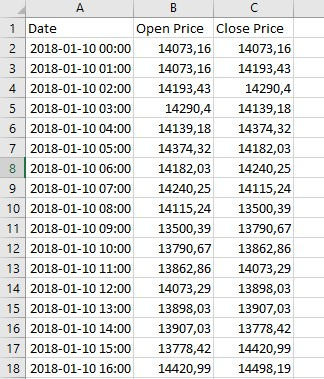
\includegraphics[width=.4\textwidth]{bitcoin}
	\caption{Bitcoin-Kursverlauf}
	\label{fig:bitcoin-course}
\end{figure}

In welchem Format die Bitcoin-Kurse vorliegen ist in Abbildung \ref{fig:bitcoin-course} zu sehen.
\newline
Den Bitcoin-Kursen werden im Rahmen dieser Arbeit Tweets gegen\"ubergestellt. Ein Tweet hat maximal 280 Zeichen. In Abbildung \ref{fig:tweet} ist ein Beispiel für ein Tweet zu sehen. 

\begin{figure}[htb]
	
\includegraphics[width=.5\textwidth]{tweet}
	\caption{Beispiel-Tweet}
	\label{fig:tweet}
\end{figure}

Um eine repr\"asentative Stichprobe zu haben, wurden knapp 120.000 Tweets untersucht. Neben dem Text eines Tweets, werden außerdem Informationen \"uber denjenigen ausgelesen, der den Tweet verfasst hat, wann diese Kurznachricht verfasst wurde, eine eindeutige Identifikationsnummer, retweets und jede Menge andere Informationen. F\"ur diese Arbeit wurde jedoch nur das Erstellungsdatum und der Text eines Tweets gesammelt. Allgemein wurden nur Nachrichten aufgezeichnet, in dessen die Zeichen: ''Bitcoin'', ''\#Bitcoin'' und ''cryptocurrency'' vorkommen.
Außerdem sind nur Tweets erfasst worden, die innerhalb der USA und einem Großteil von Kanada ver\"offentlicht wurden.
Da die Sentiment-Analyse am effizientesten funktioniert, wenn alle zu untersuchenden Texte in einer Sprache sind, wurde mit Hilfe einer Bibliothek f\"ur jeden einzelnen Tweets die entsprechende Sprache ermittelt. Alle Nachrichten, die nicht in der Sprache Englisch waren, wurden daraufhin aus dem Datensatz entfernt.